

\tikzset{every picture/.style={line width=0.75pt}} %set default line width to 0.75pt        

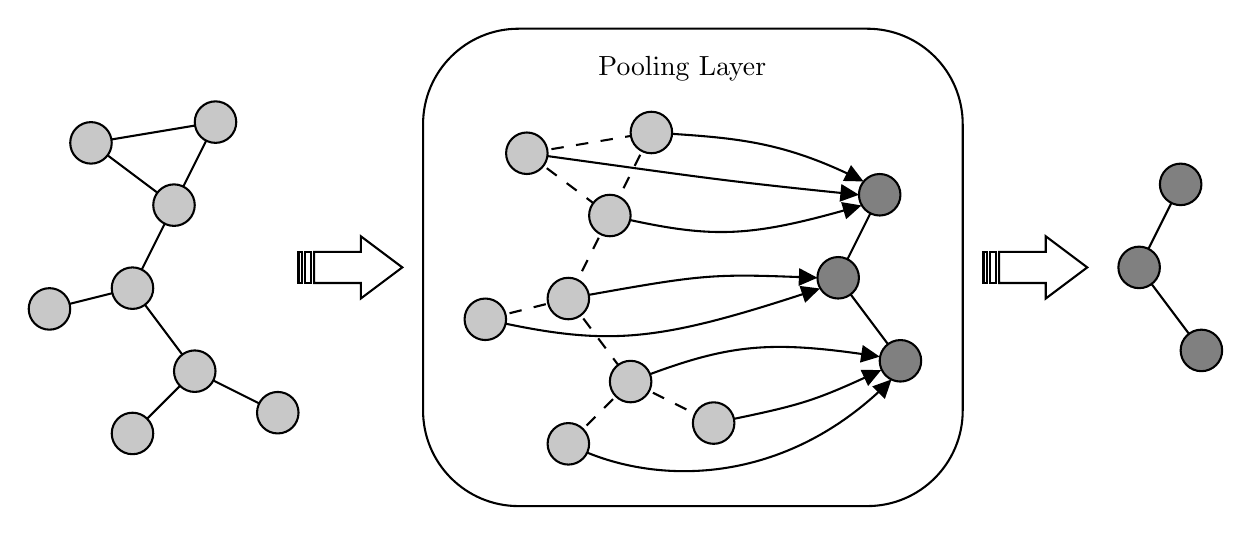
\begin{tikzpicture}[x=0.75pt,y=0.75pt,yscale=-1,xscale=1]
%uncomment if require: \path (0,300); %set diagram left start at 0, and has height of 300

%Straight Lines [id:da5096617344365821] 
\draw    (585,95) -- (565,135) ;
%Straight Lines [id:da9932827718765578] 
\draw    (565,135) -- (595,175) ;
%Curve Lines [id:da6905034262446312] 
\draw    (270,80) .. controls (352.62,91.31) and (359.81,92.89) .. (427.92,99.79) ;
\draw [shift={(430,100)}, rotate = 185.77] [fill={rgb, 255:red, 0; green, 0; blue, 0 }  ][line width=0.08]  [draw opacity=0] (8.93,-4.29) -- (0,0) -- (8.93,4.29) -- cycle    ;
%Curve Lines [id:da8335321724765272] 
\draw    (330,70) .. controls (368.17,72.52) and (391.5,73.29) .. (429.83,92.38) ;
\draw [shift={(432.2,93.58)}, rotate = 207] [fill={rgb, 255:red, 0; green, 0; blue, 0 }  ][line width=0.08]  [draw opacity=0] (8.93,-4.29) -- (0,0) -- (8.93,4.29) -- cycle    ;
%Curve Lines [id:da31100259312110135] 
\draw    (250,160) .. controls (309.35,173.29) and (331.51,171.46) .. (408.84,145.96) ;
\draw [shift={(411.2,145.18)}, rotate = 521.6700000000001] [fill={rgb, 255:red, 0; green, 0; blue, 0 }  ][line width=0.08]  [draw opacity=0] (8.93,-4.29) -- (0,0) -- (8.93,4.29) -- cycle    ;
%Curve Lines [id:da5677680537011585] 
\draw    (320,190) .. controls (366.25,171.95) and (385.37,169.74) .. (437.59,177.63) ;
\draw [shift={(440,178)}, rotate = 188.76] [fill={rgb, 255:red, 0; green, 0; blue, 0 }  ][line width=0.08]  [draw opacity=0] (8.93,-4.29) -- (0,0) -- (8.93,4.29) -- cycle    ;
%Curve Lines [id:da15435588971241] 
\draw    (360,210) .. controls (401.63,201.4) and (406.71,200.23) .. (438.22,185.63) ;
\draw [shift={(440.7,184.48)}, rotate = 515.05] [fill={rgb, 255:red, 0; green, 0; blue, 0 }  ][line width=0.08]  [draw opacity=0] (8.93,-4.29) -- (0,0) -- (8.93,4.29) -- cycle    ;
%Curve Lines [id:da7751491360366476] 
\draw    (290,220) .. controls (327.57,239.78) and (391.65,242.62) .. (444.11,190.57) ;
\draw [shift={(445.7,188.98)}, rotate = 494.49] [fill={rgb, 255:red, 0; green, 0; blue, 0 }  ][line width=0.08]  [draw opacity=0] (8.93,-4.29) -- (0,0) -- (8.93,4.29) -- cycle    ;
%Curve Lines [id:da9997311294079065] 
\draw    (310,110) .. controls (358.71,121.25) and (375.45,121.18) .. (428.74,105.88) ;
\draw [shift={(431.2,105.17)}, rotate = 523.85] [fill={rgb, 255:red, 0; green, 0; blue, 0 }  ][line width=0.08]  [draw opacity=0] (8.93,-4.29) -- (0,0) -- (8.93,4.29) -- cycle    ;
%Curve Lines [id:da5516088460235944] 
\draw    (290,150) .. controls (356.19,138.11) and (357.67,137.93) .. (407.68,139.91) ;
\draw [shift={(410,140)}, rotate = 182.27] [fill={rgb, 255:red, 0; green, 0; blue, 0 }  ][line width=0.08]  [draw opacity=0] (8.93,-4.29) -- (0,0) -- (8.93,4.29) -- cycle    ;
%Straight Lines [id:da42002527970780945] 
\draw    (60,75) -- (100,105) ;
%Straight Lines [id:da9625123729833738] 
\draw    (120,65) -- (100,105) ;
%Straight Lines [id:da011564512705323882] 
\draw    (60,75) -- (120,65) ;
%Straight Lines [id:da591791700605113] 
\draw    (100,105) -- (80,145) ;
%Straight Lines [id:da0520483680630226] 
\draw    (40,155) -- (80,145) ;
%Straight Lines [id:da243342242168614] 
\draw    (80,145) -- (110,185) ;
%Straight Lines [id:da29763945544745907] 
\draw    (110,185) -- (80,215) ;
%Straight Lines [id:da041191991130072436] 
\draw    (110,185) -- (150,205) ;
%Shape: Circle [id:dp7340107223648733] 
\draw  [fill={rgb, 255:red, 200; green, 200; blue, 200 }  ,fill opacity=1 ] (50,75) .. controls (50,69.48) and (54.48,65) .. (60,65) .. controls (65.52,65) and (70,69.48) .. (70,75) .. controls (70,80.52) and (65.52,85) .. (60,85) .. controls (54.48,85) and (50,80.52) .. (50,75) -- cycle ;
%Shape: Circle [id:dp00026389043378993726] 
\draw  [fill={rgb, 255:red, 200; green, 200; blue, 200 }  ,fill opacity=1 ] (110,65) .. controls (110,59.48) and (114.48,55) .. (120,55) .. controls (125.52,55) and (130,59.48) .. (130,65) .. controls (130,70.52) and (125.52,75) .. (120,75) .. controls (114.48,75) and (110,70.52) .. (110,65) -- cycle ;
%Shape: Circle [id:dp5553734560288552] 
\draw  [fill={rgb, 255:red, 200; green, 200; blue, 200 }  ,fill opacity=1 ] (90,105) .. controls (90,99.48) and (94.48,95) .. (100,95) .. controls (105.52,95) and (110,99.48) .. (110,105) .. controls (110,110.52) and (105.52,115) .. (100,115) .. controls (94.48,115) and (90,110.52) .. (90,105) -- cycle ;
%Shape: Circle [id:dp7685657012179221] 
\draw  [fill={rgb, 255:red, 200; green, 200; blue, 200 }  ,fill opacity=1 ] (70,145) .. controls (70,139.48) and (74.48,135) .. (80,135) .. controls (85.52,135) and (90,139.48) .. (90,145) .. controls (90,150.52) and (85.52,155) .. (80,155) .. controls (74.48,155) and (70,150.52) .. (70,145) -- cycle ;
%Shape: Circle [id:dp8225576337985958] 
\draw  [fill={rgb, 255:red, 200; green, 200; blue, 200 }  ,fill opacity=1 ] (30,155) .. controls (30,149.48) and (34.48,145) .. (40,145) .. controls (45.52,145) and (50,149.48) .. (50,155) .. controls (50,160.52) and (45.52,165) .. (40,165) .. controls (34.48,165) and (30,160.52) .. (30,155) -- cycle ;
%Shape: Circle [id:dp8048870433512154] 
\draw  [fill={rgb, 255:red, 200; green, 200; blue, 200 }  ,fill opacity=1 ] (100,185) .. controls (100,179.48) and (104.48,175) .. (110,175) .. controls (115.52,175) and (120,179.48) .. (120,185) .. controls (120,190.52) and (115.52,195) .. (110,195) .. controls (104.48,195) and (100,190.52) .. (100,185) -- cycle ;
%Shape: Circle [id:dp3899524469262352] 
\draw  [fill={rgb, 255:red, 200; green, 200; blue, 200 }  ,fill opacity=1 ] (70,215) .. controls (70,209.48) and (74.48,205) .. (80,205) .. controls (85.52,205) and (90,209.48) .. (90,215) .. controls (90,220.52) and (85.52,225) .. (80,225) .. controls (74.48,225) and (70,220.52) .. (70,215) -- cycle ;
%Shape: Circle [id:dp40591726527712235] 
\draw  [fill={rgb, 255:red, 200; green, 200; blue, 200 }  ,fill opacity=1 ] (140,205) .. controls (140,199.48) and (144.48,195) .. (150,195) .. controls (155.52,195) and (160,199.48) .. (160,205) .. controls (160,210.52) and (155.52,215) .. (150,215) .. controls (144.48,215) and (140,210.52) .. (140,205) -- cycle ;
%Straight Lines [id:da673763044302859] 
\draw  [dash pattern={on 4.5pt off 4.5pt}]  (270,80) -- (310,110) ;
%Straight Lines [id:da9124441607803917] 
\draw  [dash pattern={on 4.5pt off 4.5pt}]  (330,70) -- (310,110) ;
%Straight Lines [id:da03995998781592447] 
\draw  [dash pattern={on 4.5pt off 4.5pt}]  (270,80) -- (330,70) ;
%Straight Lines [id:da8129344208516425] 
\draw  [dash pattern={on 4.5pt off 4.5pt}]  (310,110) -- (290,150) ;
%Straight Lines [id:da6336124502461815] 
\draw  [dash pattern={on 4.5pt off 4.5pt}]  (250,160) -- (290,150) ;
%Straight Lines [id:da8022108969555355] 
\draw  [dash pattern={on 4.5pt off 4.5pt}]  (290,150) -- (320,190) ;
%Straight Lines [id:da3098627478952969] 
\draw  [dash pattern={on 4.5pt off 4.5pt}]  (320,190) -- (290,220) ;
%Straight Lines [id:da14837892723690072] 
\draw  [dash pattern={on 4.5pt off 4.5pt}]  (320,190) -- (360,210) ;
%Shape: Circle [id:dp42990613199323735] 
\draw  [fill={rgb, 255:red, 200; green, 200; blue, 200 }  ,fill opacity=1 ] (260,80) .. controls (260,74.48) and (264.48,70) .. (270,70) .. controls (275.52,70) and (280,74.48) .. (280,80) .. controls (280,85.52) and (275.52,90) .. (270,90) .. controls (264.48,90) and (260,85.52) .. (260,80) -- cycle ;
%Shape: Circle [id:dp2754617992158239] 
\draw  [fill={rgb, 255:red, 200; green, 200; blue, 200 }  ,fill opacity=1 ] (320,70) .. controls (320,64.48) and (324.48,60) .. (330,60) .. controls (335.52,60) and (340,64.48) .. (340,70) .. controls (340,75.52) and (335.52,80) .. (330,80) .. controls (324.48,80) and (320,75.52) .. (320,70) -- cycle ;
%Shape: Circle [id:dp21321858378283642] 
\draw  [fill={rgb, 255:red, 200; green, 200; blue, 200 }  ,fill opacity=1 ] (300,110) .. controls (300,104.48) and (304.48,100) .. (310,100) .. controls (315.52,100) and (320,104.48) .. (320,110) .. controls (320,115.52) and (315.52,120) .. (310,120) .. controls (304.48,120) and (300,115.52) .. (300,110) -- cycle ;
%Shape: Circle [id:dp5661953542799116] 
\draw  [fill={rgb, 255:red, 200; green, 200; blue, 200 }  ,fill opacity=1 ] (280,150) .. controls (280,144.48) and (284.48,140) .. (290,140) .. controls (295.52,140) and (300,144.48) .. (300,150) .. controls (300,155.52) and (295.52,160) .. (290,160) .. controls (284.48,160) and (280,155.52) .. (280,150) -- cycle ;
%Shape: Circle [id:dp5442339392428344] 
\draw  [fill={rgb, 255:red, 200; green, 200; blue, 200 }  ,fill opacity=1 ] (240,160) .. controls (240,154.48) and (244.48,150) .. (250,150) .. controls (255.52,150) and (260,154.48) .. (260,160) .. controls (260,165.52) and (255.52,170) .. (250,170) .. controls (244.48,170) and (240,165.52) .. (240,160) -- cycle ;
%Shape: Circle [id:dp00011290407505515354] 
\draw  [fill={rgb, 255:red, 200; green, 200; blue, 200 }  ,fill opacity=1 ] (310,190) .. controls (310,184.48) and (314.48,180) .. (320,180) .. controls (325.52,180) and (330,184.48) .. (330,190) .. controls (330,195.52) and (325.52,200) .. (320,200) .. controls (314.48,200) and (310,195.52) .. (310,190) -- cycle ;
%Shape: Circle [id:dp518700726149034] 
\draw  [fill={rgb, 255:red, 200; green, 200; blue, 200 }  ,fill opacity=1 ] (280,220) .. controls (280,214.48) and (284.48,210) .. (290,210) .. controls (295.52,210) and (300,214.48) .. (300,220) .. controls (300,225.52) and (295.52,230) .. (290,230) .. controls (284.48,230) and (280,225.52) .. (280,220) -- cycle ;
%Shape: Circle [id:dp5730004415356564] 
\draw  [fill={rgb, 255:red, 200; green, 200; blue, 200 }  ,fill opacity=1 ] (350,210) .. controls (350,204.48) and (354.48,200) .. (360,200) .. controls (365.52,200) and (370,204.48) .. (370,210) .. controls (370,215.52) and (365.52,220) .. (360,220) .. controls (354.48,220) and (350,215.52) .. (350,210) -- cycle ;
%Straight Lines [id:da001623419930635972] 
\draw    (440,100) -- (420,140) ;
%Straight Lines [id:da015699553757238416] 
\draw    (420,140) -- (450,180) ;
%Shape: Circle [id:dp36211696768410073] 
\draw  [fill={rgb, 255:red, 128; green, 128; blue, 128 }  ,fill opacity=1 ] (430,100) .. controls (430,94.48) and (434.48,90) .. (440,90) .. controls (445.52,90) and (450,94.48) .. (450,100) .. controls (450,105.52) and (445.52,110) .. (440,110) .. controls (434.48,110) and (430,105.52) .. (430,100) -- cycle ;
%Shape: Circle [id:dp01799126024681974] 
\draw  [fill={rgb, 255:red, 128; green, 128; blue, 128 }  ,fill opacity=1 ] (410,140) .. controls (410,134.48) and (414.48,130) .. (420,130) .. controls (425.52,130) and (430,134.48) .. (430,140) .. controls (430,145.52) and (425.52,150) .. (420,150) .. controls (414.48,150) and (410,145.52) .. (410,140) -- cycle ;
%Shape: Circle [id:dp058899920078356205] 
\draw  [fill={rgb, 255:red, 128; green, 128; blue, 128 }  ,fill opacity=1 ] (440,180) .. controls (440,174.48) and (444.48,170) .. (450,170) .. controls (455.52,170) and (460,174.48) .. (460,180) .. controls (460,185.52) and (455.52,190) .. (450,190) .. controls (444.48,190) and (440,185.52) .. (440,180) -- cycle ;
%Shape: Circle [id:dp5649766452502909] 
\draw  [fill={rgb, 255:red, 128; green, 128; blue, 128 }  ,fill opacity=1 ] (575,95) .. controls (575,89.48) and (579.48,85) .. (585,85) .. controls (590.52,85) and (595,89.48) .. (595,95) .. controls (595,100.52) and (590.52,105) .. (585,105) .. controls (579.48,105) and (575,100.52) .. (575,95) -- cycle ;
%Shape: Circle [id:dp5246365191278834] 
\draw  [fill={rgb, 255:red, 128; green, 128; blue, 128 }  ,fill opacity=1 ] (555,135) .. controls (555,129.48) and (559.48,125) .. (565,125) .. controls (570.52,125) and (575,129.48) .. (575,135) .. controls (575,140.52) and (570.52,145) .. (565,145) .. controls (559.48,145) and (555,140.52) .. (555,135) -- cycle ;
%Shape: Circle [id:dp5766159917435185] 
\draw  [fill={rgb, 255:red, 128; green, 128; blue, 128 }  ,fill opacity=1 ] (585,175) .. controls (585,169.48) and (589.48,165) .. (595,165) .. controls (600.52,165) and (605,169.48) .. (605,175) .. controls (605,180.52) and (600.52,185) .. (595,185) .. controls (589.48,185) and (585,180.52) .. (585,175) -- cycle ;
%Rounded Rect [id:dp6303563718720424] 
\draw   (220,66) .. controls (220,40.59) and (240.59,20) .. (266,20) -- (434,20) .. controls (459.41,20) and (480,40.59) .. (480,66) -- (480,204) .. controls (480,229.41) and (459.41,250) .. (434,250) -- (266,250) .. controls (240.59,250) and (220,229.41) .. (220,204) -- cycle ;
%Striped Right Arrow [id:dp8981402107639092] 
\draw   (167.5,127.5) -- (190,127.5) -- (190,120) -- (210,135) -- (190,150) -- (190,142.5) -- (167.5,142.5) -- cycle ;\draw   (160,127.5) -- (161.5,127.5) -- (161.5,142.5) -- (160,142.5) -- cycle ;\draw   (163,127.5) -- (166,127.5) -- (166,142.5) -- (163,142.5) -- cycle ;
%Striped Right Arrow [id:dp4519194983259933] 
\draw   (497.5,127.5) -- (520,127.5) -- (520,120) -- (540,135) -- (520,150) -- (520,142.5) -- (497.5,142.5) -- cycle ;\draw   (490,127.5) -- (491.5,127.5) -- (491.5,142.5) -- (490,142.5) -- cycle ;\draw   (493,127.5) -- (496,127.5) -- (496,142.5) -- (493,142.5) -- cycle ;

% Text Node
\draw (303,32) node [anchor=north west][inner sep=0.75pt]   [align=left] {Pooling Layer};


\end{tikzpicture}